\chapter{Creazione View}\label{chapter:View}
\section{Utilizzo di Figma per disegno interfacce}
La prototipazione delle interfacce grafiche è stata realizzata mediante l'utilizzo del software Figma\cite{Figma}.
Figma è una web application che permette di disegnare interfacce grafiche, con la possibilità di creare prototipi interattivi.
Un aspetto non secondario è la possibilità di esportare le interfacce sia in formato vettoriale che con codice CSS.
Questo aspetto, unito all'utilizzo di \ac{IA} generativa,ha permesso la conversione di interfacce grafiche in codice
 C\# Markup, con un notevole risparmio di tempo.
 Si è scelto in un primo momento di prototipare solo le interfacce principali,
 quali la schermata di login, ricerca e dettagli di prodotti, clienti e preventivi.
 Cercandi di mantenere lo scopo progettuale rivolto alla cross-platform,
  si è deciso di realizzare le interfacce in modo da essere responsive,
 e con un layout mobile first. Si è quindi cercato di inserire tutti comandi escludendo
 l'utilizzzo della tastiera e mouse, in quanto non sempre disponibili su dispositivi mobile.
 Sfruttando la compilazione condizionale, si è cercato di adattare le interfacce grafiche alle diverse piattaforme.
 Alcuni filtri sono ad esempio colassati in un menu a tendina su mobile, mentre su desktop sono sempre visibili.
 Nelle immagini che seguono si può osservare l'evoluzione dal prototipo in figura\ref{fig:Prototipo Home Figma}, 
 alla realizzazione finale delle interfacce grafiche in figura\ref{fig:Interfaccia Desktop & Mobile}.
 \begin{figure}[h]
    \centering
    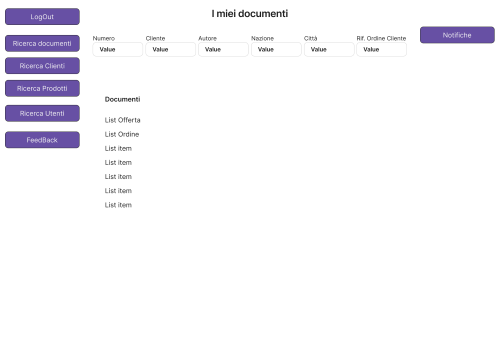
\includegraphics[width=0.6\linewidth]{figures/Figma.png}
    \caption{Prototipo Home Figma}\label{fig:Prototipo Home Figma}
\end{figure}
 \begin{figure}[h]
    \centering
    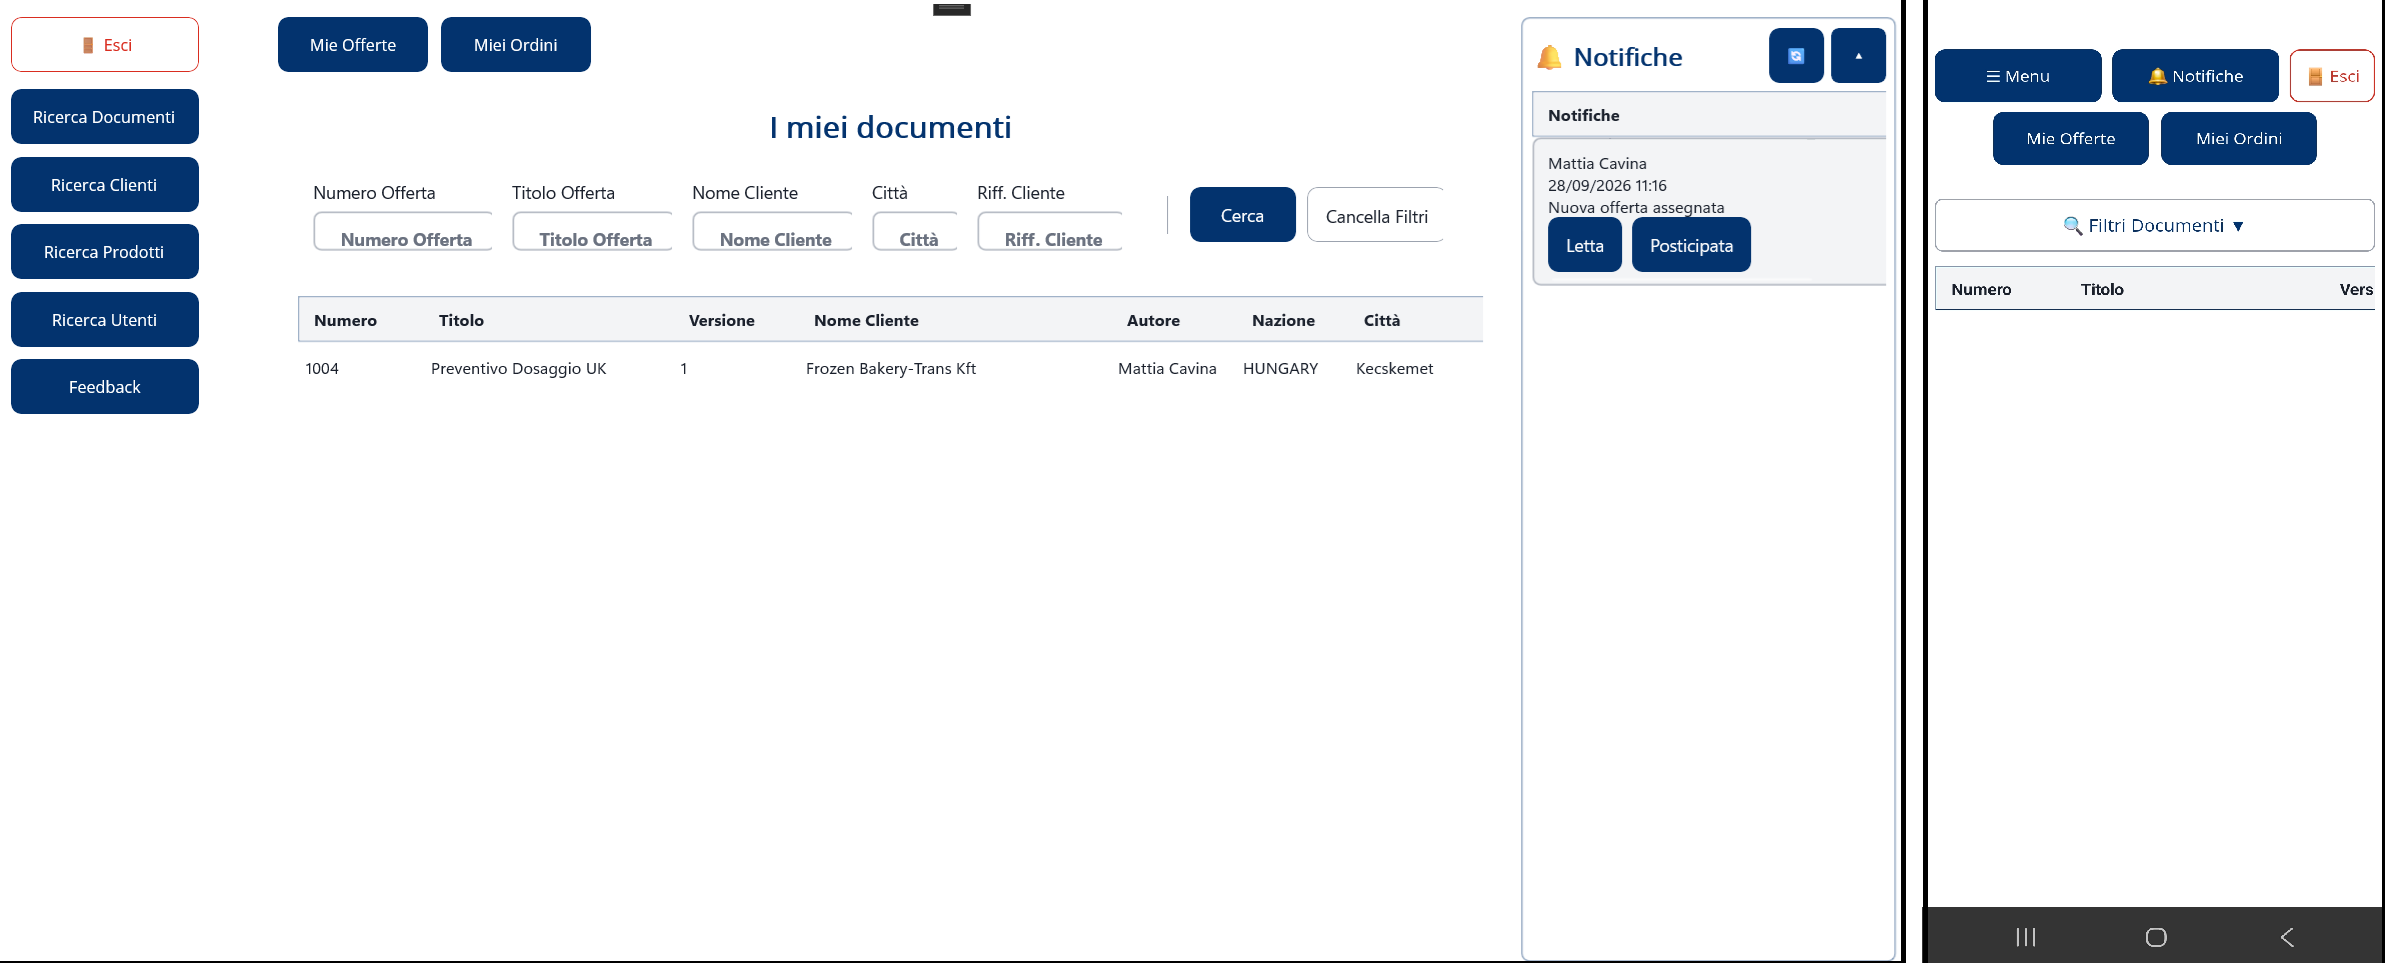
\includegraphics[width=0.6\linewidth]{figures/Realizzazione.png}
    \caption{Interfaccia Desktop & Mobile}\label{fig:Interfaccia Desktop & Mobile}
\end{figure}
 \section{Creazione delle Factory per le View}
 Dalla versione prototipale, si è deciso fin dall'inizio di realizzare
  le interfacce grafiche mediante l'utilizzo del pattern Factory.
  Questo approccio ha permesso di astrarre la creazione delle interfacce grafiche, unificando
  i metodi di creazione delle view, e permettendo di gestire le interfacce grafiche in un unico package.
  Le factory principali realizzate sono le seguenti:
\begin{itemize}
    \item \textbf{Colori:} Factory che espone i colori utilizzati nell'applicativo,
    permettendo di centralizzare la gestione dei colori.
    \item \textbf{Componenti:} Factory che espone i componenti grafici, come bottoni, etichette e caselle di testo.
    \item \textbf{Dimensioni:} Factory che espone le dimensioni dei componenti grafici, come larghezza e altezza tipica dei componenti.
    \item \textbf{PopUp di notifica:} Factory che espone i metodi per la creazione di popup di notifica,
     come messaggi di errore o di conferma.
\end{itemize}
\section{Scelta delle classi di ViewModel}